\chapter{Kerangka Arsitektur The Open Group (TOGAF)}

\section{Apa itu Kerangka TOGAF?}

\begin{figure}[h]
	\begin{center}
		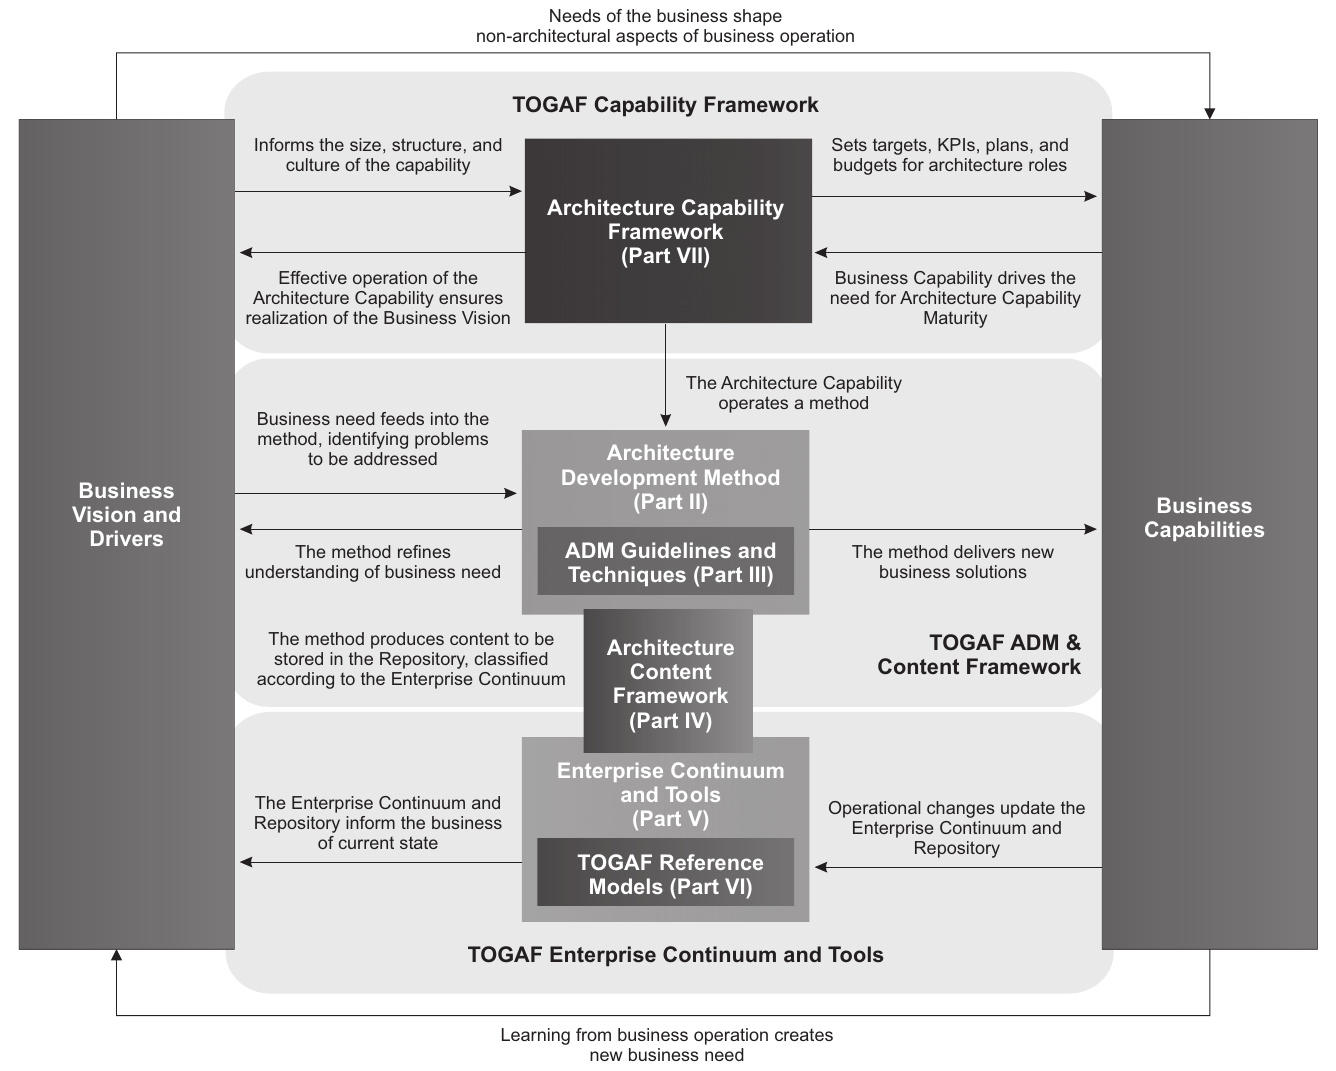
\includegraphics[width=\textwidth]{../figures/togaf}
		\caption{Kerangka Arsitektur The Open Group (TOGAF)}
	\end{center}
\end{figure}

TOGAF adalah sebuah kerangka kerja untuk pengembangan arsitektur perusahaan, yang dikembangkan oleh The Open Group, sebuah konsorsium industri TI. Ini terdiri dari metode dan alat untuk membantu dalam desain, implementasi, dan manajemen arsitektur perusahaan, dengan fokus pada manajemen siklus hidup arsitektur. TOGAF menggunakan pendekatan siklus hidup yang dapat diulang dan iteratif.

\section{Domain Arsitektur}
Kerangka TOGAF mencakup beberapa domain arsitektur: Arsitektur Bisnis berfokus pada strategi bisnis, tata kelola, organisasi, dan proses bisnis utama. Arsitektur Data menangani struktur data logis dan fisik organisasi, serta manajemen data aset dan sumber daya. Arsitektur Aplikasi menyediakan cetak biru untuk sistem aplikasi individu yang akan diterapkan, interaksinya, dan hubungannya dengan proses bisnis inti organisasi. Arsitektur Teknologi mencakup kemampuan perangkat lunak dan perangkat keras yang diperlukan untuk mendukung penerapan aplikasi bisnis, data, dan layanan, termasuk infrastruktur TI, middleware, jaringan, komunikasi, pemrosesan, dan standar.

\section{Komponen TOGAF}
Kerangka TOGAF mencakup berbagai komponen seperti Visi dan Penggerak Bisnis, Kemampuan Bisnis, Kerangka Kemampuan Arsitektur, Metode Pengembangan Arsitektur, dan Pedoman serta Teknik ADM.

Komponen tambahan TOGAF termasuk Kerangka Tata Kelola Arsitektur, Kerangka Konten Arsitektur, Deliverables, Artefak, dan Blok Bangunan, Kontinum dan Alat Perusahaan, serta Repository Arsitektur. Model Referensi TOGAF juga memainkan peran penting dalam mendefinisikan dan membimbing arsitektur perusahaan.

\section{Visi dan Penggerak Bisnis di TOGAF}
Visi bisnis menggambarkan tujuan dan pandangan masa depan sebuah organisasi. Penggerak bisnis adalah faktor yang memicu perubahan dalam sebuah organisasi. TOGAF memanfaatkan visi bisnis dan penggerak untuk membantu mendefinisikan arsitektur perusahaan. Selama fase Preliminary dan Architecture Vision dari ADM, penggerak ini membantu dalam membentuk dan membimbing arsitektur. Penggerak bisnis dapat mencakup perubahan teknologi, pergeseran pasar, atau persyaratan regulasi.

\section{Kemampuan Bisnis di TOGAF}
Kemampuan bisnis adalah kombinasi dari orang, proses, dan teknologi yang memungkinkan sebuah organisasi untuk mencapai tujuannya. TOGAF menganggap kemampuan bisnis sebagai bagian integral dari arsitektur perusahaan. Memahami kemampuan ini membantu dalam merancang dan menerapkan arsitektur yang efektif. Kemampuan bisnis diidentifikasi dan didefinisikan sepanjang proses ADM, membantu dalam desain dan eksekusi arsitektur.

\section{Kerangka Kemampuan Arsitektur TOGAF}
TOGAF 9 menyediakan Kerangka Kemampuan Arsitektur, yang mencakup materi referensi dan pedoman untuk membangun fungsi arsitektur dalam sebuah organisasi. Kerangka ini terdiri dari tujuh kategori: membangun kemampuan arsitektur, dewan arsitektur, kepatuhan arsitektur, kontrak arsitektur, tata kelola arsitektur, model kematangan arsitektur, dan kerangka keterampilan arsitektur. Kategori-kategori ini mencakup kemampuan yang diperlukan untuk menghasilkan arsitektur perusahaan yang efektif dan membantu mengidentifikasi serta mengatasi kekurangan.

\begin{figure}
	\begin{center}
		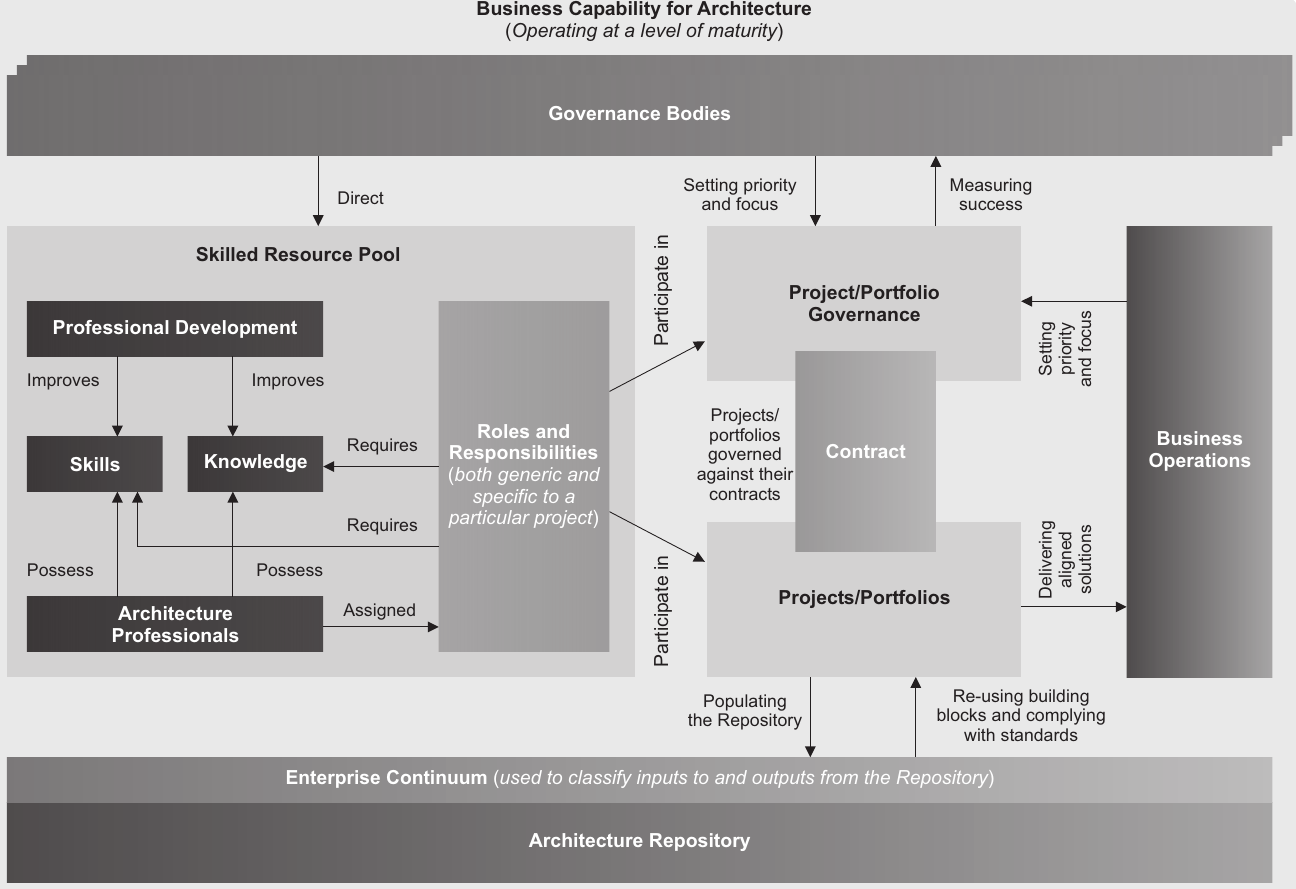
\includegraphics[width=\textwidth]{../figures/architecture_capability_framework}
		\caption{Kerangka Kemampuan Arsitektur}
	\end{center}
\end{figure}

\section{Isi Kerangka Kemampuan Arsitektur TOGAF}
Membuat Arsitektur Kemampuan melibatkan penataan struktur, proses, dan peran untuk mendukung praktik arsitektur organisasi, termasuk cakupan, pemangku kepentingan, dan tata kelola. Dewan Arsitektur mengawasi pembentukan dan operasi Dewan Arsitektur perusahaan. Kepatuhan Arsitektur memastikan bahwa arsitektur organisasi sesuai dengan standar, kebijakan, dan peraturan yang relevan. Kontrak Arsitektur mendefinisikan cakupan, tujuan, dan hasil.

\section{Isi Kerangka Kemampuan Arsitektur TOGAF (2)}
Komponen tambahan dari Kerangka Kemampuan Arsitektur termasuk Tata Kelola Arsitektur, yang memastikan keselarasan arsitektur dengan strategi dan tujuan bisnis. Model Kematangan Arsitektur membantu organisasi menilai dan meningkatkan praktik arsitektur mereka. Kerangka Keterampilan Arsitektur menyediakan peran, keterampilan, dan norma pengalaman untuk pekerjaan arsitektur.

\section{Metode Pengembangan Arsitektur (ADM)}
ADM adalah proses yang direkomendasikan oleh TOGAF untuk mengembangkan arsitektur perusahaan. Ini melibatkan fase yang terorganisir yang membantu dalam merancang, merencanakan, menerapkan, dan mengelola arsitektur perusahaan. Fase-fase ini termasuk Visi Arsitektur, Desain Bisnis, Desain Informasi, Desain Teknologi, dan Implementasi. ADM mengelola seluruh siklus hidup arsitektur perusahaan dan menawarkan pedoman serta teknik untuk setiap fase.

\begin{figure}
	\begin{center}
		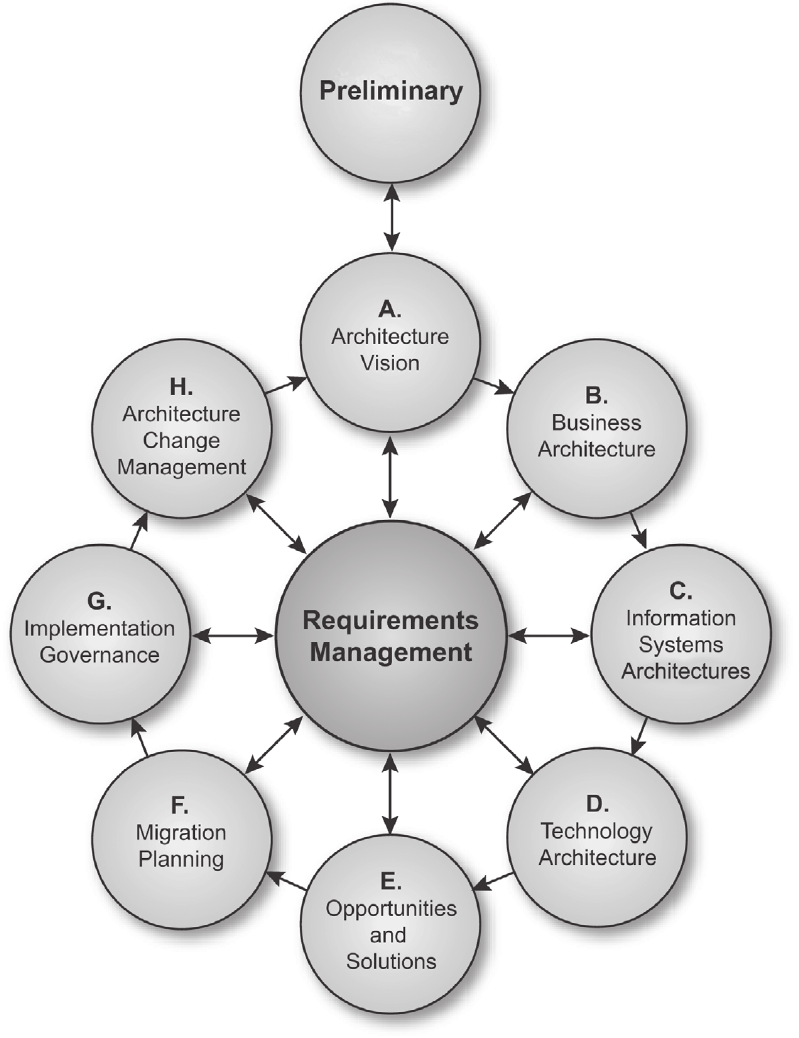
\includegraphics[width=.50\textwidth]{../figures/architecture_development_method}
		\caption{Metode Pengembangan Arsitektur}
	\end{center}
\end{figure}

\section{Pedoman dan Teknik ADM}
TOGAF menyediakan pedoman dan teknik untuk mendukung pelaksanaan ADM. Pedoman ini membantu organisasi menyesuaikan ADM dengan kebutuhan dan konteks spesifik mereka, memastikan proses tetap fokus dan efektif. Teknik umum termasuk analisis prinsip, analisis pemangku kepentingan, analisis kesenjangan, skenario bisnis, rencana migrasi, interoperabilitas, manajemen risiko, dan rencana kemampuan.

\section{Kerangka Tata Kelola Arsitektur}
Tata kelola arsitektur melibatkan pengelolaan dan pengendalian arsitektur perusahaan. TOGAF menyediakan Kerangka Tata Kelola Arsitektur yang mencakup struktur organisasi, peran dan tanggung jawab, proses, dan metode komunikasi. Kerangka ini memastikan bahwa semua proyek selaras dengan arsitektur perusahaan dan strategi bisnis, serta melibatkan pemeliharaan artefak seperti prinsip arsitektur, model, dan peta jalan.

\section{Kerangka Konten Arsitektur}
Kerangka Konten Arsitektur mendefinisikan jenis konten arsitektur yang diperlukan untuk mencakup seluruh domain bisnis. Ini memandu identifikasi, organisasi, dan pengembangan artefak arsitektur. Kerangka ini terdiri dari Deliverables, Artefak, dan Blok Bangunan. Deliverables adalah hasil yang diberikan kepada pemangku kepentingan, Artefak menggambarkan arsitektur, dan Blok Bangunan adalah komponen dari sistem bisnis atau TI.

\section{Deliverables, Artefak, dan Blok Bangunan di TOGAF}
Deliverables adalah hasil pekerjaan arsitektur yang diberikan kepada pemangku kepentingan. Artefak adalah bagian dari Deliverables yang menggambarkan arsitektur secara rinci. Blok Bangunan adalah komponen fisik, logis, atau konseptual dari sistem bisnis atau TI. Contohnya termasuk Dokumen Visi Arsitektur, Diagram Data, dan komponen server atau basis data.

\begin{figure}
	\begin{center}
		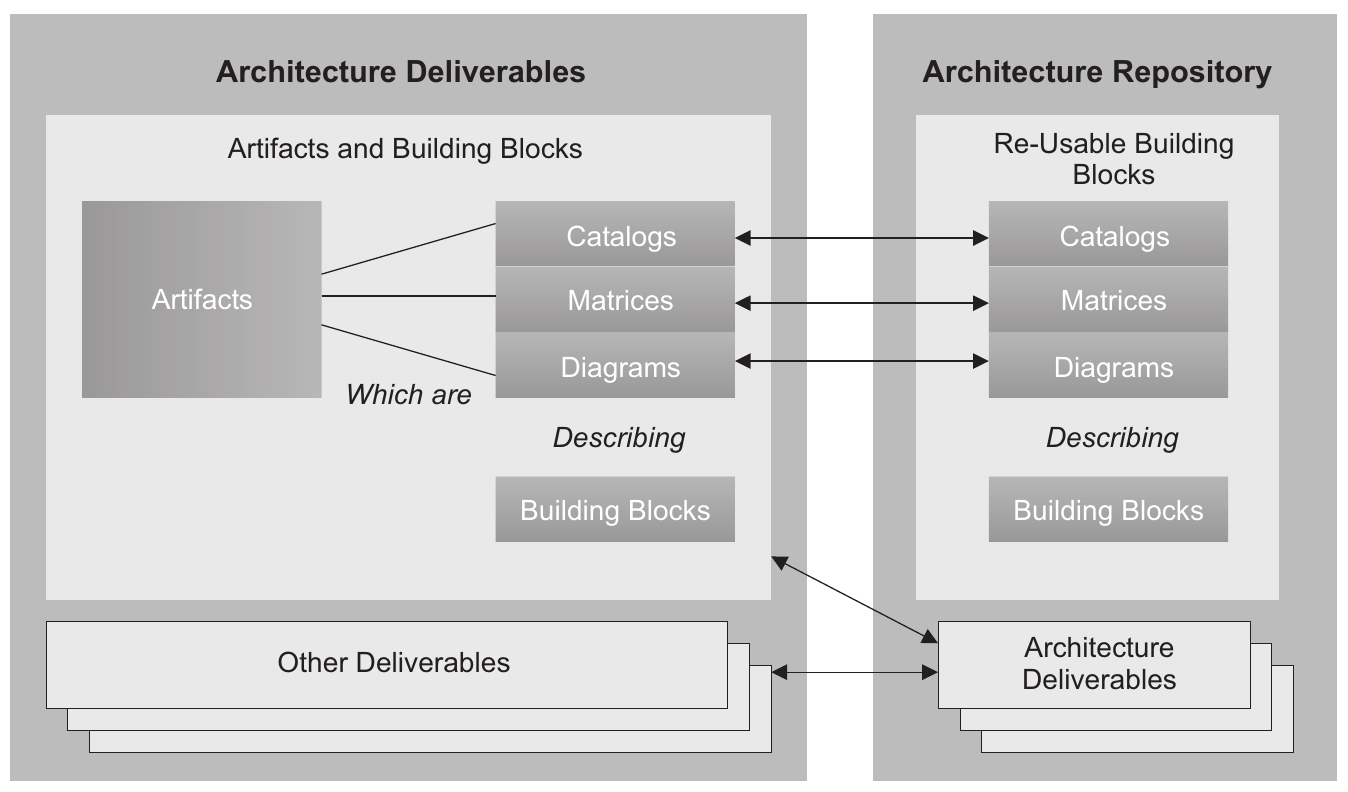
\includegraphics[width=\textwidth]{../figures/architecture_deliverables}
		\caption{Deliverables Arsitektur dan Repository Arsitektur}
	\end{center}
\end{figure}

\section{Kontinum dan Alat Perusahaan}
Kontinum Perusahaan adalah perspektif pada arsitektur dan solusi, mengkategorikan dan mengorganisir artefak. Alat TOGAF membantu dalam membuat, menganalisis, dan mengelola artefak arsitektur, memastikan pekerjaan arsitektur yang efektif dan efisien sepanjang proses ADM.

\section{Repository Arsitektur}
Repository Arsitektur adalah koleksi terstruktur dari artefak arsitektur yang berfungsi sebagai referensi bagi arsitek dan pemangku kepentingan. Ini mencakup prinsip arsitektur, model referensi, dan pola, memastikan bahwa pekerjaan arsitektur terorganisir, konsisten, dan dapat digunakan kembali.

\section{Model Referensi TOGAF}
TOGAF mencakup model referensi untuk membimbing pengembangan arsitektur perusahaan. Model-model ini menyediakan kerangka kerja dan praktik terbaik yang distandarisasi, seperti Model Referensi Teknis TOGAF dan Model Referensi Infrastruktur Informasi Terpadu, membantu memastikan konsistensi dan keselarasan dengan standar industri.

\section{Aktivitas Kelas dan Tugas}
Setelah mengumpulkan 30 literatur, lanjutkan dengan membaca, mengelompokan, dan menyimpulkan makalah-makalah tersebut. Identifikasi apa kontribusi makalah-makalah tersebut terhadap pembangunan Arsitektur Enterprise yang sedang Anda bangun. Identifikasi juga hal-hal apa saja yang membedakan makalah-makalah tersebut dengan kapabilitas Arsitektur Enterprise yang sedang Anda bangun. Tuangkan ke hasil analisis ke dalam makalah.
